\section{Desgin}%
\label{sec:desgin}

\iffalse
这一张将写本系统是如何设计的,主要内容分为两部分:一部分是如何hook。另外一部分是如何实现对各种数据结构的保护。

本文的特权特指就是内存管理,管理VMCS的原因就是里边含有EPTP,其余的域并不进行保护。

那么文章的核心就是剥夺了VMM管理物理内存的权限,这就是HyperPS的P的内容。
那么针对这一特点,这一思路,设计要怎么写。
要说明如下的几个问题:1. 如何分离权限,即VMM管理内存都是靠什么实现的,特权的实现途径是啥,怎么将这些特权分离。这里要写出两个东西:1.1 原本的VMM对内存管理的相关函数被Hook,所有的操作都无法在VMM中实施,即完成了HOOK。1.2 为了防止攻击者直接修改EPT paging structure,这就是将EPT从常规的空间中移除。
这两个点要顺序换过来,先写移除,再写hook。
2. 第二要写怎么实现保护,在hook完成后,剥离了VMM对物理内存的管理,HyperPS是如何实现对内存的管理的。这里要假如关于缺页中断的相关内容,怎么处理EPT异常,也要处理新建EPT的内容,也要包括不同虚拟机的映射关系,也要绑定EPT与VM的关系,不允许VM和VMM更改EPTP内容。

上面的1 2就是两段的内容,首先要给出一个overview,讲整个框架的结构。

##################
开头内容中文初稿
##################
这一节,我们首先提出我们的HyperPS,我们详细描述HyperPS的构成组件。然后我们详细阐述了HyperPS是如何剥离原VMM对内存的管理权限的。最后我们提出HyperPS是如何实现对内存的保护,从而实现保护虚拟机的运行以抵御一个受危害的VMM。
讲HyperPS如何实现对物理内存的管理。
\fi
In this section, we first propose the architecture of HyperPS. Then, in the following subsection, we elaborate on how HyperPS stripped the compromised HostOS kernel's privilege of managing guest VM's memory and the physical memory. Finally, we illustrate how HyperPS manages the guest VM's memory and physical memory to resist the compromised HostOS/Hypervisor.


\subsection{HyperPS Overview}%
\label{sub:hyperps_overview}

% 首先一句话说明HyperPS要做什么,然后Figure depict the details on the architecture of HyperPS.
% As shown in Figure, 我们创造了一个同层隔离空间用于履行原本属于compromised HostOS的管理虚拟机物理内存的权力。


% We present HyperPS to protect guest virtual machines against compromised Hypervisor. In virtualization environment, the hyperivor deprivileges the guest VM’s kernel and interposes all interactions between guest VMs and the physical memory. Neither isolation between VMs nor virtual-physical mapping relationships in a VM will inevitable be tamperred if the Hypervisor has been compromised. HyperPS, thus, deprives the Hypervisor of privileges on managing physical memory.

In a virtualization environment, the HostOS/Hypervisor deprivileges the guest VM’s kernel and interposes all interactions between guest VMs and the physical memory. 
If the HostOS/Hypervisor has been compromised, both isolation between VMs and virtual-physical mapping relationships for a VM will inevitablely be tampered. 
Thus, in this paper, we present HyperPS to deprive the Hypervisor of privileges on managing physical memory.

% Neither isolation between VMs nor virtual-physical mapping relationships in a VM will inevitable be tamperred if the Hypervisor has been compromised.

Figure \ref{fig:design} depicts the details on the architecture of HyperPS. 
Firstly, as shown in Figure \ref{fig:design}, we create a delicate kernel-level secure and isolated execution space, called HyperPS Space, to inherit privileges of managing physical memory that originally belonged to the compromised Hypervisor. 
Original functions about physical memory management in the compromised Hypervisor, such as EPT operations, EPTP switching operations, and some VMCS operations, are hooked into the HyperPS Space. 
However, there are still some cases where attackers subvert memory management data structures by using regular memory access. Attackers can also bypass the hooked functions by introducing new malicious VMX assembly code. HyperPS, in consideration of these cases, removed VMCS and EPT from the original Hypervisor space and placed them in the HyperPS Space. 
% For cases where attackers subvert memory management data structures by using regular memory access, and cases where attackers bypass the hooked functions by introducing new malicious VMX assembly code
% use regular memory access to tamper with
% For cases where an attacker uses regular memory access or newly introduced malicious VMX assembly code to bypass the hooked functions and tamper with the relevant memory management data structures, HyperPS removed VMCS and EPT, which are crucial to virtualization, from the original Hypervisor space and places them in the HyperPS Space.
Secondly, in the HyperPS Space, we introduce two new data structures, called Page-Mark structure and VM-Mark structure, to tag the mapping relations between the physical frames and the virtual machines. With the help of these two data structures, even if an attacker attempts to tamper EPT Paging-structures with malicious value through a legal function invocation, HyperPS can still effectively detect such attacks and resist them.
Lastly, Switch Gate is the only interface between the Normal Space and the HyperPS Space.

%FIXME 图中的内容添加虚拟机退出的线,removed的字段加粗 pptt是表 修改成表的形式

\begin{figure*}[htpb]
    \centering
    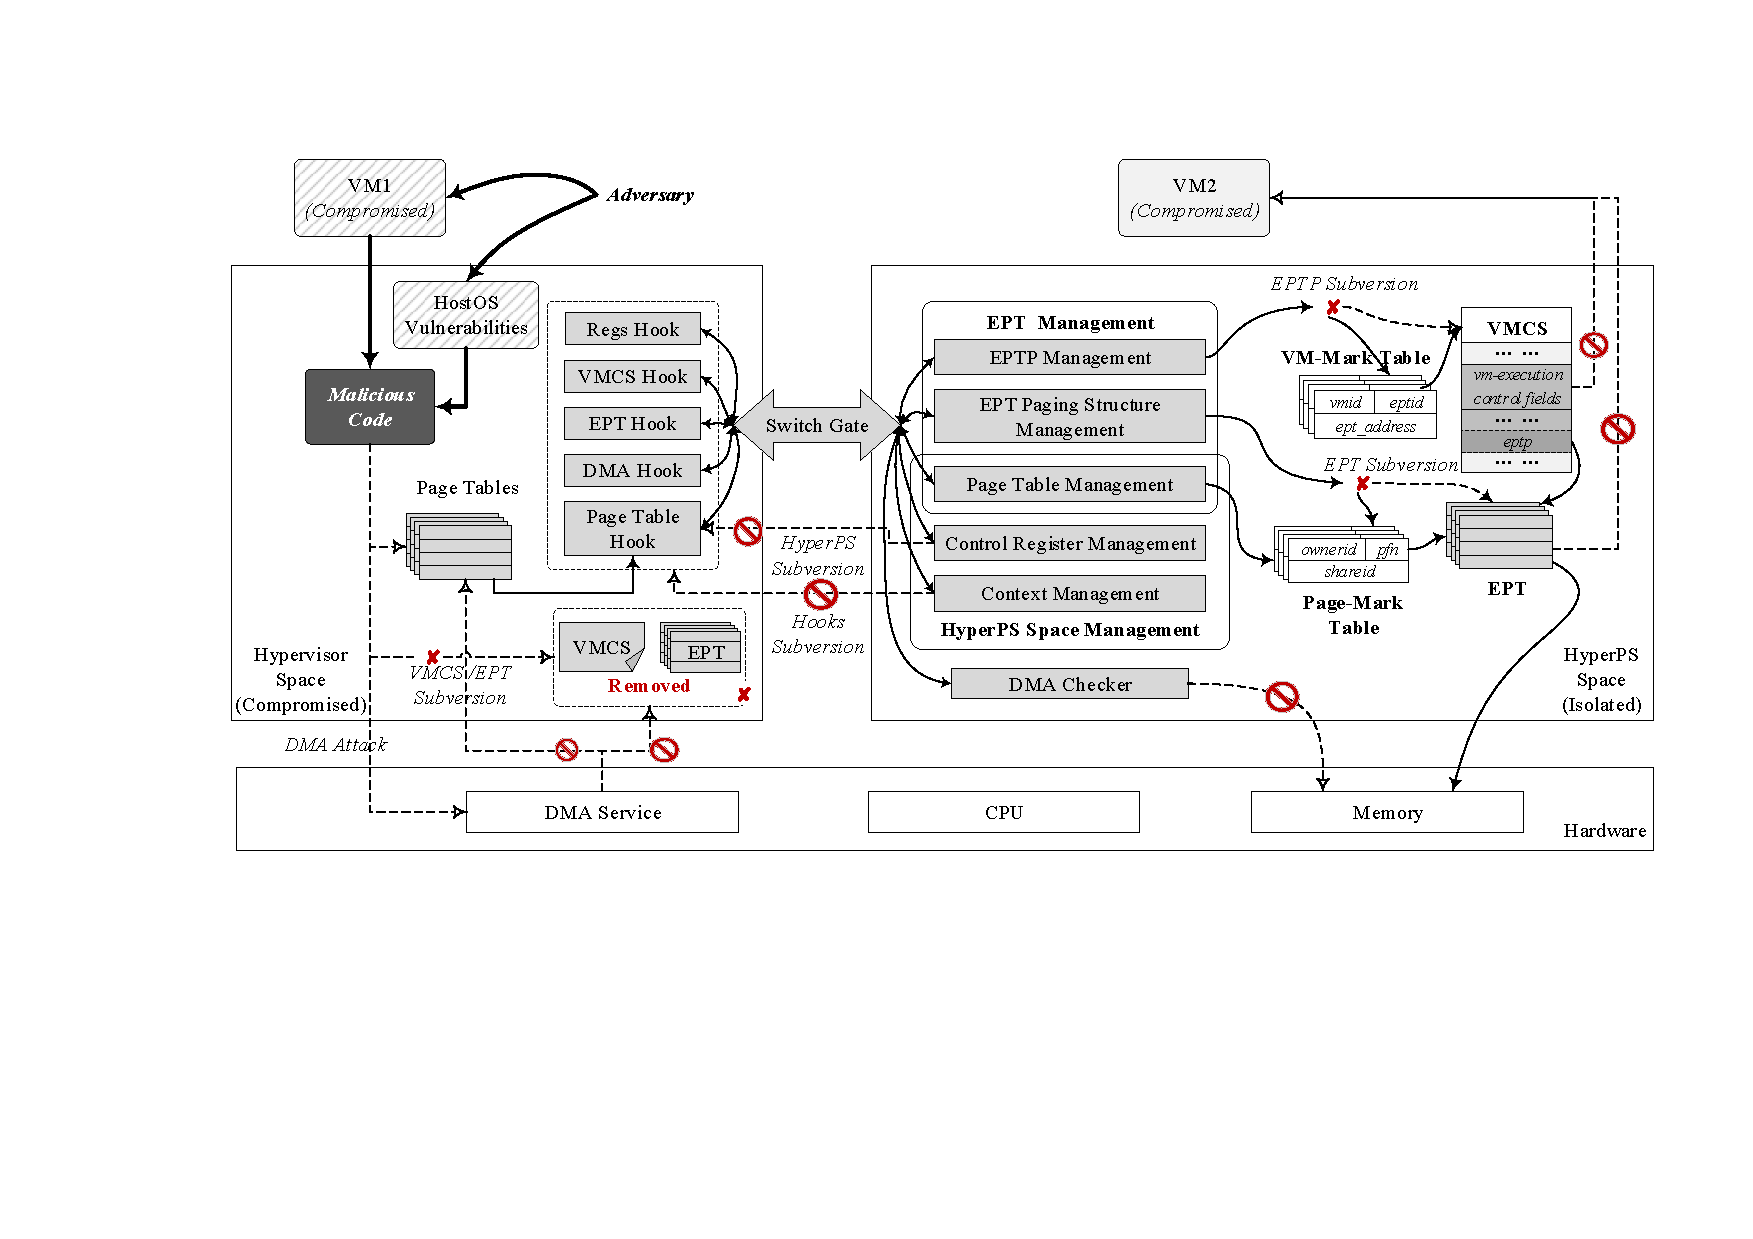
\includegraphics[width=0.9\linewidth]{IMG/newdesign.pdf}
    \caption{HyperPS Architecture  \\ HyperPS is committed to protect guest virtual machine under the compromised HostOS/Hypervisor. Privileges to manage VMCS and EPT are stripped from the compromised HostOS/Hypervisor into a separated and secure execution environment: HyperPS Space. The HyperPS Space shares the same processor privilege as the HostOS. HyperPS does not rely on any special hardware or a higher privilege. Updates to VMCS and EPT are abandoned by the HyperPS, if the operations are not authorized or are adjudged as harmful to virtual machine.}%
    \label{fig:design}
\end{figure*}



\iffalse
那么文章的核心就是剥夺了VMM管理物理内存的权限,这就是HyperPS的P的内容。
那么针对这一特点,这一思路,设计要怎么写。
要说明如下的几个问题:1. 如何分离权限,即VMM管理内存都是靠什么实现的,特权的实现途径是啥,怎么将这些特权分离。这里要写出两个东西:1.1 原本的VMM对内存管理的相关函数被Hook,所有的操作都无法在VMM中实施,即完成了HOOK。1.2 为了防止攻击者直接修改EPT paging structure,这就是将EPT从常规的空间中移除。
这两个点要顺序换过来,先写移除,再写hook。
2. 第二要写怎么实现保护,在hook完成后,剥离了VMM对物理内存的管理,HyperPS是如何实现对内存的管理的。这里要假如关于缺页中断的相关内容,怎么处理EPT异常,也要处理新建EPT的内容,也要包括不同虚拟机的映射关系,也要绑定EPT与VM的关系,不允许VM和VMM更改EPTP内容。
\fi

\subsection{Privilege Separation}%
\label{sub:privilege_separation}

\iffalse
首先要讲管理内存的权限是通过EPT实现的,要实现特权的分离,分为两步,一是将EPT从原有空间移除,使得原有的Hypervisor无法直接access数据结构。第二步是对能access这些数据结构的函数进行验证。
% 将移除操作这些数据结构的逻辑。
在传统的没有HyperPS的虚拟化环境中,Hypervisor 通过EPT直接管理管理内存
这里要先讲为什么要将EPT和VMCS从原有的空间移除,然后再讲怎么移除。移除以后存在疑问,就是会造成PANIC, 如何解决,就是hook的问题,
The EPT mechanism is a feature that can be used to support the virtualization of physical memory. 
EPT defines a layer of address translation that augments the translation of linear addresses. 
When EPT is in use, certain addresses that would normally be treated as physical addresses (and used to access memory) are instead treated as guest-physical addresses. Guest-physical addresses are translated by traversing a set of EPT paging structures to produce physical addresses that are used to access physical memory.
It's EPT mechanism that treat guest-physical address like a virtual address and the EPTP is the CR3.
We should write (\verb|VMWRITE|) EPTP to the VMCS. 
\fi

% According to the Intel manual, the EPT mechanism is a core feature that is used to support the virtualization of physical memory.
EPT defines a layer of address translation that augments the translation of linear addresses. 
When EPT is in use, the EPT interposes all memory access between guest VMs and the physical memory. 
Certain addresses that would normally be treated as physical addresses (and used to access memory) are instead treated as guest-physical addresses. Guest-physical addresses are translated by traversing a set of EPT paging structures to produce physical addresses that are used to access memory.
% If the hyperivor has been subverted by the attacker,
If attackers have gained control over a Hypervisor, 
neither isolation between VMs nor virtual-physical mapping relationships in a VM are immune to them. 
% Attackers can modify any EPT paging structures with any values.
In this paper, HyperPS deprives the Hypervisor's privileges of managing physical memory by limiting it from accessing and managing all EPTs. 
Figure \ref{fig:inter} depicts the difference in the VM-Exit handling between the traditional system and the system with HyperPS.
\begin{figure}[htpb]
    \centering
    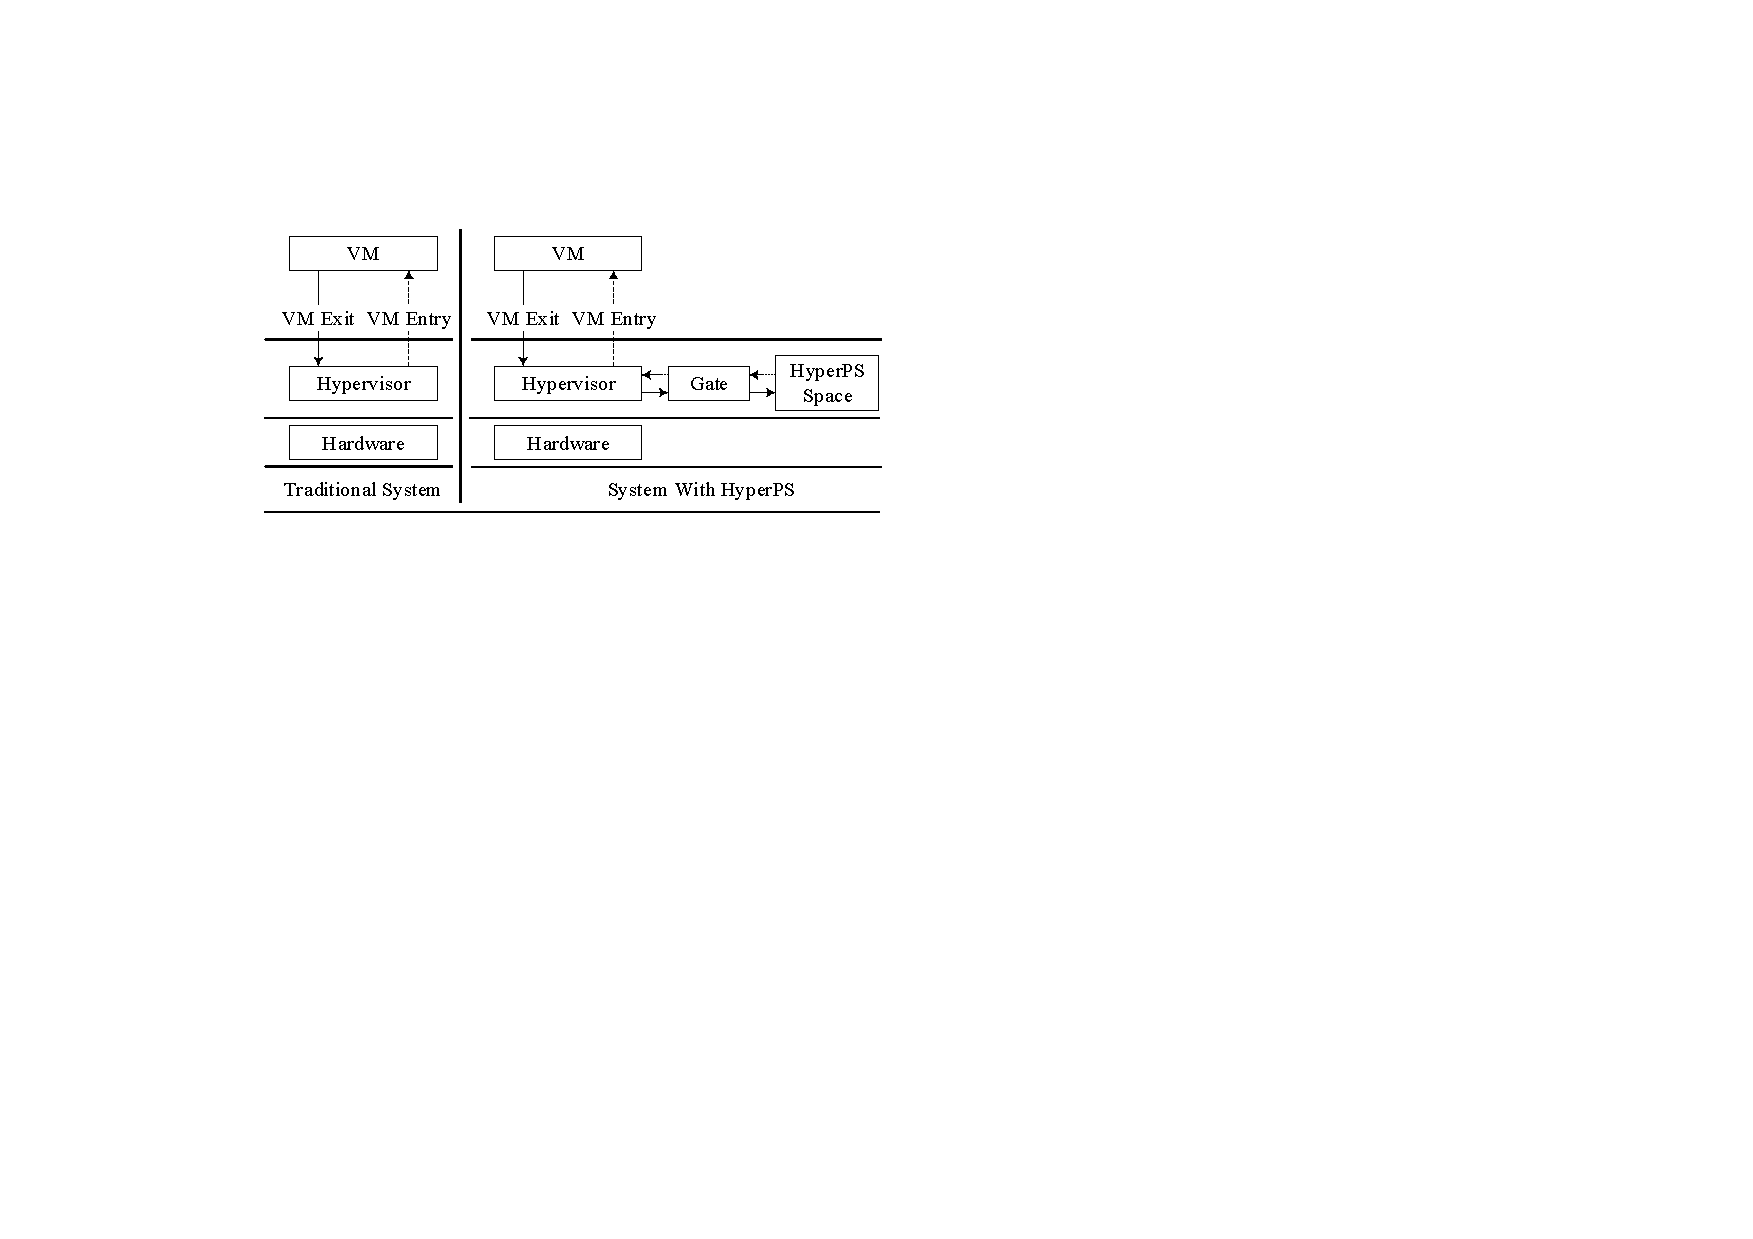
\includegraphics[width=0.8\linewidth]{IMG/interaction.pdf}
    \caption{Interaction Difference between the traditional system and system with HyperPS \\ VM-Exit handling only involves the Hypervisor in traditional system. In the system with HyperPS, VM-Exit is redirect into the HyperPS Space through the Gate. Context Management during VM-Exit and VM-Entry is managed by the HyperPS.}%
    \label{fig:inter}
\end{figure}


% Exception handle
% all code and any data in guest
% any VM's content in memory can no longer be
% EPT paging structures
% neither isolation between VMs nor virtual-physical mapping relationships in a VM
% nor
% In this paper, HyperPS deprives the compromised hyperivor with privileges of managing physical memory by limiting it from accessing and managing all EPTs.
% deprives the virtual machine
% 上面的内容说明了要限制权限是通过EPT来实现的。怎么移除EPT 为什么要移除VMCS
\iffalse
首先要讲管理内存的权限是通过EPT实现的,要实现特权的分离,分为两步,一是将EPT从原有空间移除,使得原有的Hypervisor无法直接access数据结构。第二步是对能access这些数据结构的函数进行验证。
% 将移除操作这些数据结构的逻辑。
在传统的没有HyperPS的虚拟化环境中,Hypervisor 通过EPT直接管理管理内存
这里要先讲为什么要将EPT和VMCS从原有的空间移除,然后再讲怎么移除。移除以后存在疑问,就是会造成PANIC, 如何解决,就是hook的问题,
It's EPT mechanism that treat guest-physical address like a virtual address and the EPTP is the CR3.
we should write (VMWRITE) EPTP to the VMCS. 
\fi


Firstly, HyperPS removed all EPTs and VMCSes from the Hypervisor space. EPT manages all physical memory of the VM, as mentioned above, HyperPS removed them from the Hypervisor space. However, there is a hardware register, called Extended Page Table Pointer (EPTP), that contains the address of the base of EPT table, as well as EPT configuration information. Simple obliteration of EPT would make EPTP error which will crash the whole virtualization environment too. 
Besides, the VMCS records the value of EPTP in the VM-Execution Control Fields. The processor will load the value in that field into the hardware register when VM-Entry. 
Even if the attacker cannot directly tamper with EPTs, he can also subvert the guest VMs by tampering with a malicious EPTP value in the VMCS. Thus, HyperPS removed all VMCSes from the Hypervisor too. 
% The adversary can tamper with the EPTP value in the VMCS to make the VM use a new set of malicious EPT table.
% Thus, HyperPS
% A Hypervisor load the value
% EPTP is a hardware register that works like the CR3 register in traditional memory translation. It always points to the
% The VMCS stores the value of EPTP in the VM-Execution Control Fields.
% VMCS store EPTP that points to EPT
% EPTP works like the CR3 in

Secondly,  HyperPS hooks all VMCS operation and EPT operation functions in the Hypervisor into the HyperPS Space.
In the QEMU-KVM architecture, The KVM provides a wrapper around privileged instructions and is responsible for executing privileged instructions.
The QEMU does not need to deal architecture specific details, it just needs to invoke KVM functions with proper parameters. 
HyperPS hooks KVM's VMCS and EPT functions into the HyperPS Space. In the HyperPS Space, Context Management in the HyperPS Space Management component checks the invoked parameters and verifies if the inputted parameters are legal or not.  
% Based on Intel manuals, VMCS can only be manipulated by privileged instructions: \verb|VMCLEAR| \verb|VMPTRLD|, \verb|VMREAD|, \verb|VMWRITE|, and so on.
% In the QEMU-KVM architecture, the KVM is responsible for executing these privileged instructions. The KVM provdes a wrapper around these privileged instructions. The QEMU does not need to deal architecture specific details, it just need to invoke KVM functions with proper parameters.
% For example, \verb|vmcs_writel()| wraps the privileged instruction \verb|VMWRITE|, and \verb|vmcs_readl()| wraps the privileged instruction \verb|VMREAD|.
% HyperPS hooks these functions into the HyperPS Space. In the HyperPS Space, Context Management in the HyperPS Space Management component check the invoked parameters and verifies if the write to \verb|VM-Execution Control Fields.EPTP| is legal or not.
Since VMCS is hidden in the HyperPS Space which is accessible by functions in the Hypervisor space, all context management (accessing VMCS operations) will be trapped int HyperPS Space inevitably.
% inevitablely.
%During VM-Exit (codes to access VMCS can only be executed in VM-Exit), the Hypervisor 
EPT operation functions are also hooked into the HyperPS Space too. EPT operation functions are different from VMCS operation functions, for the VMCS can only be accessed by just a few privileged instructions. Instead of hooking EPT accessing functions, HyperPS hooks all EPT operation functions. Functions about EPT creation, load, traversal, update and destruction are re-placed into the HyperPS Space. Functions that invoke these EPT operation functions are hooked into the HyperPS Space.

% operation functions
% HyperPS checks the
% provide a wrapper around these privileged instructions.
% are responsible
% HyperPS hooks functions that contain these instructions.
% In specific,
% at each time when VM exits to the Hypervisor, HyperPS
% VMCS operation and EPT operation functions certainly involve privileged instructions.
% On a privileged instruction, it switches back to the KVM kernel module,

Lastly, HyperPS also takes DMA attacks into consideration. An attacker with the ability of arbitrary memory access by exploiting DMA vulnerabilities can tamper VMCSes and EPTs. IOMMU carries out access control for DMA access. Thus, in this paper, HyperPS employs IOMMU mechanism to resist DMA attacks.
In the Hypervisor space, HyperPS found out all the critical data used by IOMMU, and removed the corresponding page table entries that map these data from the page tables. In this paper, HyperPS mainly defines the entrance address of HyperPS, the Page-Mark data, and the VM-Mark data (details about Page-Mark and VM-Mark data structure are illustrated in Section \ref{ssub:eptp_protection}) as the critical data.
In the HyperPS Space, HyperPS intercepts the address mapping function about I/O. At runtime, HyperPS verifies whether the address belongs to the HyperPS Space on receiving signals of executing these IO functions. 


% HyperPS removed all corresponding page table entries that map
% mapping of the critical data from the page table which IOMMU uses.
% In the HyperPS Space, DMA Management Component
% In this paper, HyperPS employs IOMMU mechanism to resist DMA attacks. IOMMU carries out access control for DMA access.

% \subsection{VM Memory Protection}%
% \label{sub:vm_memory_protection}
\subsection{Privilege Management}%
\label{sub:privilege_management}



\iffalse
那么文章的核心就是剥夺了VMM管理物理内存的权限,这就是HyperPS的P的内容。
那么针对这一特点,这一思路,设计要怎么写。
要说明如下的几个问题:1. 如何分离权限,即VMM管理内存都是靠什么实现的,特权的实现途径是啥,怎么将这些特权分离。这里要写出两个东西:1.1 原本的VMM对内存管理的相关函数被Hook,所有的操作都无法在VMM中实施,即完成了HOOK。1.2 为了防止攻击者直接修改EPT paging structure,这就是将EPT从常规的空间中移除。
这两个点要顺序换过来,先写移除,再写hook。
2. 第二要写怎么实现保护,在hook完成后,剥离了VMM对物理内存的管理,HyperPS是如何实现对内存的管理的。这里要假如关于缺页中断的相关内容,怎么处理EPT异常,也要处理新建EPT的内容,也要包括不同虚拟机的映射关系,也要绑定EPT与VM的关系,不允许VM和VMM更改EPTP内容。
\fi

HyperPS has removed EPTs and VMCSes from the original Hypervisor space, and functions about accessing and updating them have also been hooked into the HyperPS Space. 
The HostOS/Hypervisor has already been deprived of privileges of managing the physical memory directly. Actually, the HostOS/Hypervisor can not access EPTs and VMCSes with regular memory access instructions or DMA instructions. 
However, The HostOS/Hypervisor could still retrieve details about EPTs and VMCSes through legal functions. 
The attacker can also tamper with EPT Paging-structures and VMCS fields with malicious input to these hooked functions.
In this paper, HyperPS present two tables : Page-Mark Table and VM-Mark Table, to tag the mapping relations between the physical memory page frames and the virtual machines. Page-Mark Table consists of Page-Mark structure, while VM-Mark Table consists of VM-Mark structure.

\subsubsection{EPTP Protection}%
\label{ssub:eptp_protection}
In this paper, we propose a table: VM-Mark Table to restrict Hypervisor from loading an unverified EPTP value arbitrarily.
The VM-Mark Table consists of VM-Mark structures. 
In the Hypervisor, a new EPTP means a different EPT Paging-structure hierarchy. An attacker can map VM virtual address to a totally new physical page frame that holds malicious code. In this paper, HyperPS hooks all functions that can switch the value of EPTP and verifies if the value is authorized by HyperPS before. HyperPS relies on the VM-Mark structure to identify whether the operation of changing EPTP is legal or not. 

Table \ref{tb:vmmark} presents the basic architecture of the VM-Mark structure.
The field \verb|VMID| is a magic number randomly generated when the VM is created. 
The field \verb|EPTID| is also a magic number randomly generated when the EPTP is allocated.
In a virtualization environment,
the Hypervisor can use a different VMCS for each virtual machine that it supports. However, these VMCSes share the same EPTP value for a single VM. 
HyperPS, thus, blinds the different EPT with a VM identifier instead of each VMCS.
HyperPS also takes \verb|VMFUNC| into consideration too. EPTP switching is VM function 0. This VM function allows VM in VMX non-root operation to load a new value for the EPTP. The EPTP switching operation does not incur VM-Exit to VMX root operation.
The \verb|VMFUNC| is limited to selecting from a list of potential EPTP values configured in advance by the Hypervisor in VMX root operation. Thus, HyperPS also hooks all functions that manage the EPTP list in VMX root operation.

When the Hypervisor is going to load a new value for the EPTP or change the EPTP list in VMX root operation, functions are hooked and control flow is redirected to HyperPS Space. 
HyperPS iterates the VM-Mark table to check if the EPTP is authorized in advance.

% checks if the input EPTP value matches a entry in
% EPTP in VMX root operation or change
% In this paper, HyperPS
% EPTP switching is VM function0. This VM function allows software in VMX non-root operation to load a new value for the EPT pointer (EPTP), thereby establishing a different EPT paging-structure hierarchy. Software is limited to selecting from a list of potential EPTP values configured in advance by software in VMX root operation.
% When switching from one VM to another, the Hypervisor writes the same EPTP value into all the VMCSes for a single VM.
% These VMCSes share the same EPT
% Different VMCS that
% HyperPS blinds the EPT with the VM identifier instead of the VMCS.
% HyperPS blinds EPTs with VM identifiers

\begin{table}[]
    \caption{VM-Mark Structure}
    \resizebox{\linewidth}{!}{
\begin{tabular}{l|l|l|l}
\hline
\textbf{Label}       & \multicolumn{1}{c|}{VMID} & \multicolumn{1}{c|}{EPTID} & \multicolumn{1}{c}{EPT\_Address} \\ \hline
\textbf{Description} & The VM Identifier         & The EPT Identifier         & The Entry Address of this EPT    \\ \hline
\end{tabular}}
    \label{tb:vmmark}
\end{table}

% unauthorized EPTP
% EPTP switching is VM function0. this VM function allows software in VMX non-root operation to load a new value for the EPT pointer (EPTP), thereby establishing a different EPT paging-structure hierarchy. Software is limited to selecting from a list of potential EPTP values configured in advance by software in VMX root operation.
% VM-mark的作用是保证VM 和对应的EPT 是对应的,攻击者无法通过更换新的EPT表实现对虚拟机的攻击。
% Page-mark的作用是用于虚拟机内部的隔离。

\subsubsection{EPT Paging-structure Protection}%
\label{ssub:ept_paging_structure_protection}
Values that update to EPT Paging-structures need to be verified too. In this paper, we present Page-Mark structure to record the relationships between EPT Paging-structures and the physical memory page frames. In HyperPS Space, HyperPS composes all Page-Mark structures into one table, called Page-Mark Table.
HyperPS guarantees effective isolation between different virtual machines based on this Page-Mark Table. 

Table \ref{tb:pagemark} presents the basic architecture of the Page-Mark structure.
The field \verb|PFN| is the first address of the physical memory page frame. HyperPS fills in this field when a physical memory page frame is assigned to a VM. Usually, the Hypervisor will create a new EPT Paging-structure that maps this page frame and assigns the physical memory page frame to a guest physical memory page frame. The field \verb|OwnerID| is the same as the value of \verb|VMID| that identifies different VM/EPT. At the time when a physical memory page frame is assigned to a VM, HyperPS fills the field \verb|OwnerID| with the value of the corresponding \verb|VMID|. 
Kernel Same-page Merging (KSM), used by the KVM, allow for a greater guest density of identical or similar guest operating system by avoiding memory duplication.
% KVM guests to share identical memory pages
% However, In some virtualization environment, some particular physical memory page frames may be shared between differnt VMs.
For example, different VMs with the same kernel may share the same physical memory page frames that hold the kernel code. HyperPS takes this situation into consideration too. If one physical memory page frame is shared between VMs, HyperPS fills the field \verb|SharedID| with the one of the VM's \verb|OwnerID|.

HyperPS has hooked all functions about EPT operations.
At runtime, control flow will be redirected to the HyperPS Space when the Hypervisor invokes these functions. 
In the HyperPS, HyperPS index the Page-Mark structure tables with the physical memory page frame address. 
HyperPS ensures that any update to EPT Paging-structures must be in line with records in the Page-Mark Table.
With the help of the Page-Mark Table, the attacker can no longer map a physical memory page frame that initially belongs to a victim VM to the malicious VM. The compromised Hypervisor can not map the guest VM into a dedicated physical memory page frame anymore. 
% If the update to EPT
% HyperPS will verify the owner of pages when EPT update
% HyperPS has hooked all functions about EPT operations. On executing thses functions, control flow is redirect into the HyperPS Space.

\begin{table}[]
    \caption{Page-Mark Structure}
    \resizebox{\linewidth}{!}{
\begin{tabular}{l|l|l|l}
\hline
\textbf{Label}       & \multicolumn{1}{c|}{OwnerID} & \multicolumn{1}{c|}{SharedID} & \multicolumn{1}{c}{PFN}                                                                  \\ \hline
\textbf{Description} & The Owner Identifier         & The Shared Identifier         & \begin{tabular}[c]{@{}l@{}}The Address of the Physical \\ Memory Page Frame\end{tabular} \\ \hline
\end{tabular}}
    \label{tb:pagemark}
\end{table}



% the attribution of different physical memory page frames.



With the help of VM-Mark Table and Page-Mark Table, HyperPS can effectively protect the isolation between VMs and the correct virtual-physical mapping relationships in a VM. 


















